

\tikzset{every picture/.style={line width=0.75pt}} %set default line width to 0.75pt        

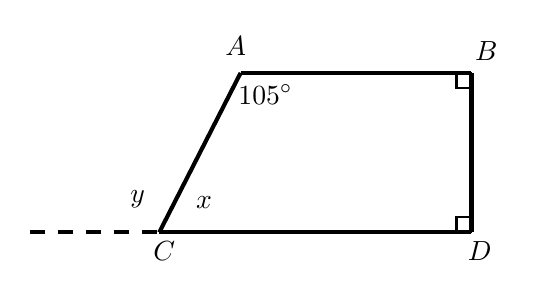
\begin{tikzpicture}[x=0.75pt,y=0.75pt,yscale=-1,xscale=1, scale=0.8]
%uncomment if require: \path (0,218); %set diagram left start at 0, and has height of 218

%Shape: Rectangle [id:dp392879367849994] 
\draw   (418,146) -- (427,146) -- (427,155) -- (418,155) -- cycle ;
%Shape: Rectangle [id:dp28556743489112235] 
\draw   (418,59) -- (427,59) -- (427,68) -- (418,68) -- cycle ;
%Straight Lines [id:da15725270794626356] 
\draw [line width=1.5]    (427,155) -- (239,155) ;


%Straight Lines [id:da6108314492525089] 
\draw [line width=1.5]    (427,155) -- (427,59) ;


%Straight Lines [id:da21099235794946036] 
\draw [line width=1.5]    (288,59) -- (427,59) ;


%Straight Lines [id:da9882398763880909] 
\draw [line width=1.5]    (239,155) -- (288,59) ;


%Straight Lines [id:da2719389491415545] 
\draw [line width=1.5]  [dash pattern={on 5.63pt off 4.5pt}]  (161,155) -- (239,155) ;



% Text Node
\draw (285,43) node   {$A$};
% Text Node
\draw (436,46) node   {$B$};
% Text Node
\draw (242,166) node   {$C$};
% Text Node
\draw (432,166) node   {$D$};
% Text Node
\draw (303,72) node   {$105^{\circ }$};
% Text Node
\draw (266,137) node   {$x$};
% Text Node
\draw (226,135) node   {$y$};


\end{tikzpicture}